\documentclass[conference]{IEEEtran}
\IEEEoverridecommandlockouts
\usepackage{cite}
\usepackage{amsmath,amssymb,amsfonts}
\usepackage{algorithmic}
\usepackage{float}
\usepackage{graphicx}
\usepackage{textcomp}
\usepackage{xcolor}
\usepackage{epsfig}
\usepackage{amsmath}
\usepackage{enumitem}
\usepackage{hyperref}
 \hypersetup{ 
     colorlinks = true, 
     citecolor = black,       
     urlcolor = cyan
     } 
\usepackage[utf8]{inputenc}
\renewcommand\IEEEkeywordsname{Keywords}

\def\BibTeX{{\rm B\kern-.05em{\sc i\kern-.025em b}\kern-.08em
    T\kern-.1667em\lower.7ex\hbox{E}\kern-.125emX}}
\begin{document}

\title{\begin{center} Comprehensive Statistical Analysis of Wisconsin Breast Cancer Data: Insights from Regression Analysis and Clustering Techniques\end{center}

}

\author{
\IEEEauthorblockN{Pedro Ferreira}
\IEEEauthorblockA{\textit{IPCA, Barcelos, Braga, Portugal} \\
a17029@alunos.ipca.pt}
\and

\IEEEauthorblockN{Enmanuel Abilheira}
\IEEEauthorblockA{\textit{IPCA, Barcelos, Braga, Portugal} \\
a16430@alunos.ipca.pt}
\and

\IEEEauthorblockN{Daniel Fernandes}
\IEEEauthorblockA{\textit{IPCA, Barcelos, Braga, Portugal} \\
a17014@alunos.ipca.pt}
}



\maketitle

\begin{abstract}
Breast cancer is a significant public health concern, and understanding its predictors and subtypes is crucial for effective diagnosis and treatment. Breast cancer remains one of the most prevalent and formidable challenges in global public health. It is the most commonly diagnosed cancer among women worldwide, with millions of new cases reported annually. Despite advancements in early detection and treatment, breast cancer continues to exact a significant toll on individuals, families, and healthcare systems. Understanding the complex factors contributing to breast cancer development, progression, and response to treatment is essential for improving patient outcomes and reducing mortality rates.

In this study, we conducted a comprehensive statistical analysis of breast cancer data from the Wisconsin Breast Cancer dataset. Focusing on regression analysis and clustering techniques, we sought to uncover key predictors of breast cancer malignancy and identify distinct subgroups within the dataset. By leveraging clinical and histological features of breast tumors, we aimed to elucidate the multifaceted nature of breast cancer and provide insights that could inform personalized treatment strategies and improve patient care.
\end{abstract}


\begin{IEEEkeywords}
Breast Cancer, Wisconsin Diagnostic Dataset, Regression Analysis, Clustering Techniques
\end{IEEEkeywords}




\vspace{0.1cm}
\section{Introduction}
Breast cancer is the most commonly diagnosed cancer among women worldwide and is a significant cause of morbidity and mortality. According to the World Health Organization (WHO), breast cancer accounted for an estimated 2.3 million new cases and 685,000 deaths globally in 2020 alone\cite{arnold2022current}.

Having replaced lung cancer as the most commonly diagnosed cancer globally, breast cancer today accounts for 1 in 8 cancer diagnoses and a total of 2.3 million new cases in both sexes combined\cite{sung2021global}.

Representing a quarter of all cancer cases in females, it was by far the most commonly diagnosed cancer in women in 2020, and its burden has been growing in many parts of the world, particularly in transitioning countries\cite{arnold2022current, heer2020global}.

Statistical analysis plays a crucial role in advancing our understanding of breast cancer and improving patient outcomes. By applying statistical methods to breast cancer research, clinicians and researchers can identify important risk factors associated with disease development and progression.
Statistical methods enable researchers to uncover hidden patterns and associations within large-scale genomic and clinical datasets. By analyzing genomic profiles and tumor characteristics, statistical techniques such as clustering and classification algorithms can identify distinct molecular subtypes of breast cancer with unique prognostic and therapeutic implications\cite{curtis2012genomic}.

\subsection{About the Dataset}

The Breast Cancer Wisconsin Diagnostic dataset is widely used in machine learning research and clinical studies. It consists of features computed from digitized images of fine needle aspirates (FNAs) of breast masses, providing valuable information for the analysis and diagnosis of breast tumors.

The dataset contains a total of 569 instances, each with 33 variables. Among these variables, the most crucial one is the diagnosis, which indicates whether the tumor is malignant (M) or benign (B). The remaining variables represent various characteristics of cell nuclei, such as radius, texture, perimeter, area, smoothness, compactness, concavity, concave points, symmetry, and fractal dimension.

The features provided in the dataset were computed based on the work described in the paper\cite{bennett1992robust}.
This dataset has undergone extensive study and utilization for cancer diagnosis and prognosis prediction.

\subsection{Data Source}

The dataset can be obtained from multiple sources, including the UCI Machine Learning Repository\cite{UCI} and Kaggle\cite{Kaggle}. It is also available through the University of Wisconsin's FTP server. The dataset is commonly referred to as the "Wisconsin Breast Cancer dataset" or "WDBC" and is publicly accessible for research purposes.

\subsection{Attributes Description}

The dataset contains several attributes, including ID numbers, diagnosis labels, and ten real-valued features computed for each cell nucleus. These features provide valuable insights into the physical dimensions, texture, and composition of the tumor cells. The mean, standard error, and "worst" (or largest) values of these features were computed for each image, resulting in a total of 30 features.

The class distribution within the dataset is imbalanced, with 357 instances labeled as benign and 212 instances labeled as malignant.

\vspace{0.2cm}
\textbf{Description:}

\begin{enumerate}
    \item ID number
    \item Diagnosis (\textit{M} = malignant, \textit{B} = benign)
    \item Ten real-valued features are computed for each cell nucleus:
    \begin{enumerate}
        \item[a)] Radius
        \item[b)] Texture (standard deviation of gray-scale values)
        \item[c)] Perimeter
        \item[d)] Area
        \item[e)] Smoothness (local variation in radius lengths)
        \item[f)] Compactness
        \item[g)] Concavity (severity of concave portions of the contour)
        \item[h)] Concave points (number of concave portions of the contour)
        \item[i)] Symmetry
        \item[j)] Fractal dimension ("coastline approximation")
    \end{enumerate}
\end{enumerate}

\vspace{0.2cm}
This dataset serves as a valuable resource for researchers and practitioners in the field of oncology, facilitating the development of predictive models and diagnostic tools for breast cancer detection and treatment.

\subsection{Goals}
The primary aim of this comprehensive analysis is to rigorously examine and identify potential predictors for breast cancer through the application of various statistical methodologies. In this particular study, three distinct statistical techniques were utilized: linear regression, logistic regression and clustering methodologies.

\vspace{0.2cm}

\subsubsection{Linear Regression}

\vspace{0.2cm}
The primary objective of applying linear regression is to model the relationship between one or more independent variables (predictors) and a dependent quantitative variable (response). Linear regression aims to find the best-fitting linear equation that describes the relationship between these variables.

Linear regression serves multiple purposes in statistical analysis. Primarily, it facilitates the comprehension of the relationship existing between independent variables and the dependent variable by quantifying this association through the estimation of slope and intercept parameters inherent in the linear equation.

Moreover, it enables the execution of statistical inference, permitting hypothesis testing on model coefficients and the evaluation of overall fit to the data. This functionality serves to ascertain the significance of relationships and the reliability of the model under examination.

\vspace{0.5cm}
\subsubsection{Logistic Regression}
The primary objective of applying logistic regression to a dataset in statistical analysis is to model the relationship between one or more independent variables (predictors) and a binary dependent variable (response). Unlike linear regression, which is suitable for continuous outcomes, logistic regression is used when the dependent variable is categorical with two levels.

Logistic regression serves multiple key purposes in statistical analysis. 
It models the probability that an observation belongs to a specific category or class, estimating this probability based on predictor variables.
Furthermore, it helps understanding how changes in independent variables relate to changes in the probability of the outcome, achieved through estimation of model coefficients.

\vspace{0.5cm}
\subsubsection{Clustering}

Clustering techniques aim to partition the dataset into groups or clusters, where observations within the same cluster are more similar to each other than to those in other clusters.

Clustering techniques play a vital role in statistical analysis by offering a multifaceted approach to understanding and analyzing datasets.
Moreover, clustering aids in pattern recognition by identifying inherent structures or clusters within the data. These patterns offer valuable insights that can inform subsequent analysis or decision-making processes.
Additionally, clustering serves as a powerful tool for anomaly detection, enabling the identification of observations that deviate significantly from established patterns.

\vspace{0.5cm}

\section{{Methodology}}
\vspace{0.2cm}
Before delineating the methodology for each of the techniques, it is imperative to note that the feature "Id" was not considered in the analysis, as it solely serves as an identifier for each record.

\subsection{Linear Regression}
\vspace{0.2cm}
\textbf{Process:}

\vspace{0.2cm}

\begin{enumerate}
    \item For the multiple linear regression (MLR) analysis, emphasis was placed on the mean attributes of the dataset. The selection of mean features was based on their capacity to represent the average value across multiple measurements, thereby offering a robust characterization of the central tendency of each attribute.
    
    \item Subsequently, the correlation between these features was examined, and the feature demonstrating the highest absolute correlation with the others was designated as the response variable.
    
    \item With the selected features, we proceeded to fit the linear model in order to assess the statistical significance of the coefficients/predictors.
    
    \item Following the linear model fitting, we executed a sequential deletion algorithm to ascertain whether a submodel exhibiting comparable or superior explanatory power with fewer predictors, in accordance with the principle of parsimony, could be attained.

    \item Furthermore, we conducted an F-test using ANOVA to compare the full model with the submodel.
    
    \item In the final submodel, the summary of the fit revealed that the coefficients of all utilized predictors possessed associated p-values below the conventional significance level of \(\alpha = 0.05\). Thus, we infer that all these predictors have statistically significant coefficients.
    
\end{enumerate}

\subsection{Logistic Regression}
\vspace{0.2cm}
\textbf{Process:}
\vspace{0.2cm}
\begin{enumerate}
    \item For the logistic regression analysis, we initiated by designating "diagnosis" as the response variable, with all remaining features serving as predictors.
    
    \item When attempting to fit the full model (encompassing all features), it was observed that the model failed to converge. This occurrence could be attributed to several factors, including elevated multicollinearity among predictors, data separation (wherein certain predictor values solely correspond to one of the possible outcome variable values, thus leading to perfect prediction), or numerical instability.
    
    \item Following this, an analysis of the correlation between these features was conducted, revealing the presence of numerous highly correlated predictor features.

    \item Moreover, a Variance Inflation Factor (VIF) analysis was performed, which quantifies the degree to which the variance of an estimated regression coefficient is inflated due to collinearity. Subsequently, it was noted that the predictors exhibited notably high VIF values.

    \item To mitigate this issue, feature selection was conducted utilizing Lasso regression. Cross-validation techniques were employed to determine the optimal lambda (regularization parameter) that minimizes cross-validation error.

    \item Subsequently, the significant features identified through Lasso regression were utilized to construct a logistic regression model.
    
    \item Following the logistic model fitting, we executed a sequential deletion algorithm to ascertain whether a submodel exhibiting comparable or superior explanatory power with fewer predictors, in accordance with the principle of parsimony, could be attained.

    \item Furthermore, we conducted an F-test using ANOVA to compare the full model with the submodel.
    
    \item In the final submodel, the summary of the fit revealed that the coefficients of all utilized predictors possessed associated p-values below the conventional significance level of \(\alpha = 0.05\). Thus, we infer that all these predictors have statistically significant coefficients.

    \item Finally, a likelihood ratio test statistic was conducted to ascertain whether removing any of these predictors would lead to a significant decrease in the model fit. It was concluded that all the predictors employed remained statistically significant in the final model.
    
\end{enumerate}

\subsection{Clustering}

\vspace{0.2cm}
\textbf{Process:}
\vspace{0.2cm}
\begin{enumerate}
    \item In the clustering analysis, all features were utilized except for the qualitative feature 'diagnosis'.
    
    \item Prior to implementing the clustering techniques, a check was conducted to determine if data scaling was necessary. It was observed that the input variables exhibited varying units of measurement and significantly different variances. Consequently, it was concluded that scaling was required.
    
    \item Two clustering techniques were employed: hierarchical clustering and k-means.
    
    \item Regarding hierarchical clustering, the Euclidean distance metric was utilized. An analysis was conducted using clValid to determine the most appropriate linkage method for our data. Following testing and analysis, it was determined that Ward's method was the most suitable linkage method for our purposes. Additionally, through examination of the dendrogram and optimal scores obtained from clValid, it was concluded that the appropriate number of clusters for our data was 2.
    
    \item Regarding k-means clustering, we assessed the optimal starting number of clusters (k) using the elbow method, silhouette method, and clValid. Following this analysis, it was determined that the most appropriate number of initial clusters (k) to yield meaningful results was 2.
    
    \item Furthermore, principal component analysis (PCA) was conducted to identify the minimum number of principal components necessary to explain more than 80\% of the variance in the data. It was determined that this minimum number of components was 5. Subsequently, hierarchical clustering and k-means were executed using this number of components.
    
\end{enumerate}
\section{{Results}}
\vspace{0.2cm}
\subsection{Linear Regression}
In this subsection, we will present and discuss the results obtained for the final linear regression model.

The model summary output is as follows:

\begin{figure}[!h]
      \centering
       {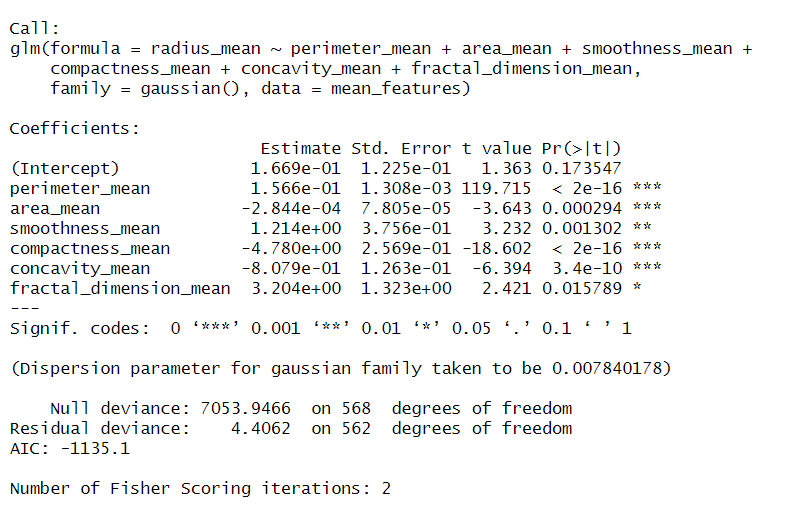
\epsfig{file = assets/mlr_final_summary.png, width = 8 cm}}
      \caption{Summary of the linear regression model}
\end{figure}


The overall model suggests that the coefficients for all predictors have associated p-values that are less than the conventional significance level of 0.05. This indicates that all predictor variables are statistically significant in explaining the variability in the response variable (radius\_mean). Therefore, we can infer that all predictors have statistically significant coefficients.

The model's goodness of fit can be evaluated by comparing the null deviance (before adding predictors) and the residual deviance (after adding predictors). A significant reduction in deviance suggests that the predictors explain a significant amount of variability in the response variable.

\vspace{0.5cm}

\textbf{Coefficients Interpretation}:
\begin{enumerate}
\item \textbf{Perimeter Mean:} For every one-unit increase in perimeter\_mean, the radius\_mean is expected to increase by 0.1566 units, on average, holding other predictors constant.
\item \textbf{Area Mean:} For every one-unit increase in area\_mean, the radius\_mean is expected to decrease by 0.0002844 units, on average, holding other predictors constant.
\item \textbf{Smoothness Mean:} For every one-unit increase in smoothness\_mean, the radius\_mean is expected to increase by 1.214 units, on average, holding other predictors constant.
\item \textbf{Compactness Mean:} For every one-unit increase in compactness\_mean, the radius\_mean is expected to decrease by 4.780 units, on average, holding other predictors constant.
\item \textbf{Concavity Mean:} For every one-unit increase in concavity\_mean, the radius\_mean is expected to decrease by 0.8079 units, on average, holding other predictors constant.
\item \textbf{Fractal Dimension Mean:} For every one-unit increase in fractal\_dimension\_mean, the radius\_mean is expected to increase by 3.204 units, on average, holding other predictors constant.
\end{enumerate}

\vspace{0.5cm}

The equation for the adjusted hyperplane of radius\_mean adjusted, based on the model summary is:

\begin{equation}
\begin{aligned}
\text{radius\_mean} &= 0.1669 + 0.1566 \times \text{perimeter\_mean}\\
&\quad - 0.0002844 \times \text{area\_mean}\\
&\quad + 1.214 \times \text{smoothness\_mean} \\
&\quad - 4.780 \times \text{compactness\_mean} \\
&\quad - 0.8079 \times \text{concavity\_mean} \\
&\quad + 3.204 \times \text{fractal\_dimension\_mean}
\end{aligned}
\end{equation}

\vspace{0.5cm}

\textbf{Sum of Squared Residuals}:
\begin{equation}
\begin{aligned}
SS_{\text{Residuals}} = \sum_{i=1}^{n} (y_i - \hat{y}_i)^2
\end{aligned}
\end{equation}

For the sum of squared residuals, the calculated value was 4.40618.

\vspace{0.5cm}

\textbf{Coefficient of Determination (R-squared)}:
\begin{equation}
\begin{aligned}
R^2 = 1 - \frac{\text{Deviance of MLR model}}{\text{Deviance of null model}}
\end{aligned}
\end{equation}

\vspace{0.5cm}
For the coefficient of determination (R-squared), the calculated value was 0.9993754.

\vspace{0.5cm}
\textbf{Residuals Analysis}:

\begin{figure}[!h]
      \centering
       {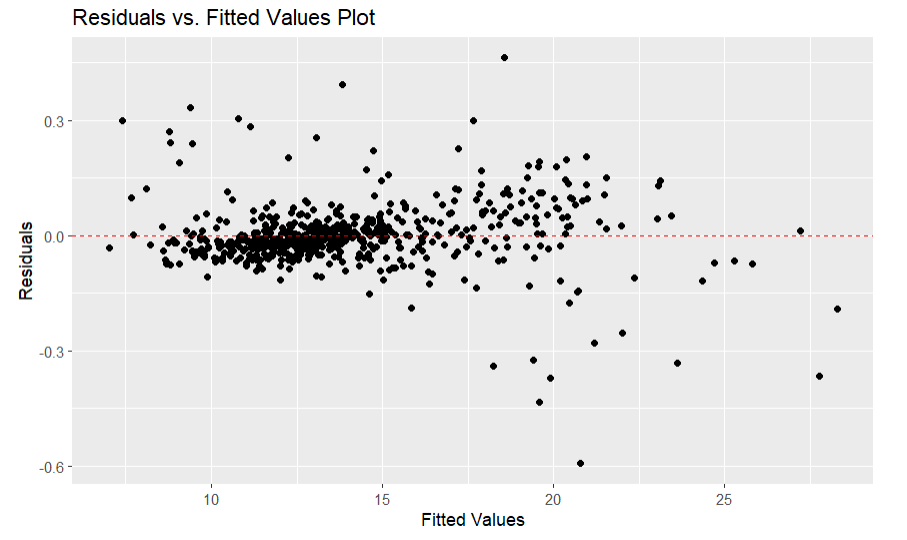
\epsfig{file = assets/mlr_residualsvsfitted.png, width = 8 cm}}
      \caption{Residuals vs. Fitted Values Plot}
      \label{fig:mlr_resvsfit}
\end{figure}

\vspace{0.5cm}

The points depicted in the plot correspond to the residuals associated with each observation within the dataset. Ideally, these residuals should exhibit a random dispersion around the horizontal line defined by y = 0.

From the plot, it is discernible that the residuals exhibit a predominantly random dispersion around the horizontal line at y = 0, exhibiting no discernible pattern as the fitted values vary, save for a  number of outliers. Notably, the spread of residuals remains consistently distributed across the spectrum of fitted values, indicating that the linear regression model adequately captures the underlying relationship between the predictors and the response variable.

\vspace{0.5cm}

\begin{figure}[!h]
      \centering
       {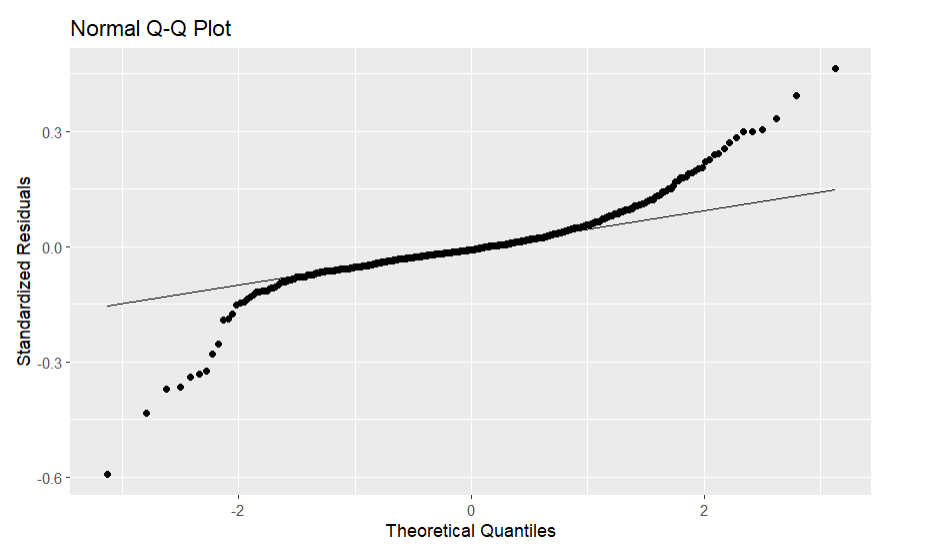
\epsfig{file = assets/mlr_qqplot.png, width = 8 cm}}
      \caption{Normal Q-Q Plot}
      \label{fig:mlr_qq}
\end{figure}

\vspace{0.5cm}

The normal Q-Q (quantile-quantile) plot is a diagnostic tool used to assess whether the distribution of the residuals from a regression model follows a normal (Gaussian) distribution.

The x-axis of the plot represents the theoretical quantiles of a standard normal distribution, while the y-axis represents the standardized residuals (residuals divided by their standard deviation), which should ideally follow a standard normal distribution if the regression model assumptions are met.

From figure \ref{fig:mlr_qq}, the observed residuals adhere to the theoretical quantiles for the most part, indicating substantial conformity to the normal distribution assumption. However, some deviations from the expected pattern are discernible at the extremities of the plot.

\vspace{0.5cm}

\begin{figure}[!h]
      \centering
       {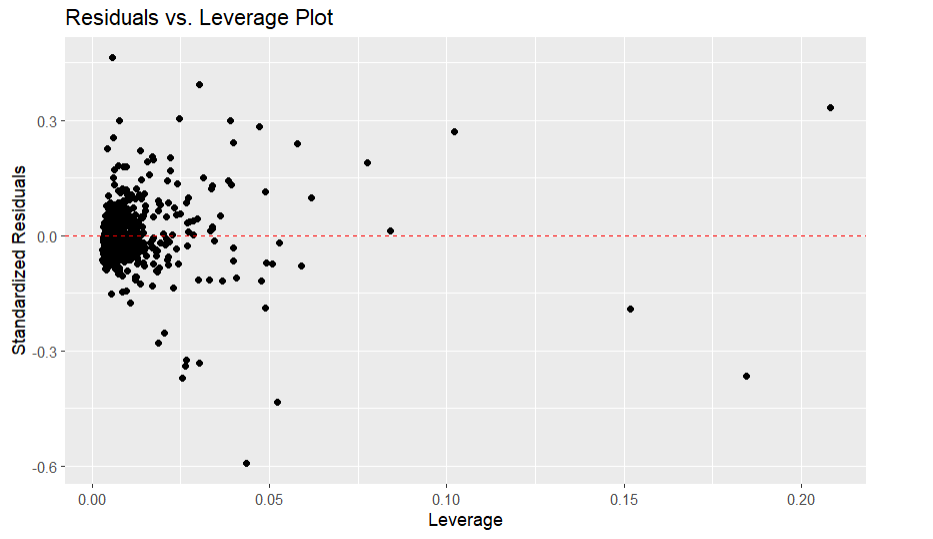
\epsfig{file = assets/mlr_std_res_vs_leverage.png, width = 8 cm}}
      \caption{Standardized Residuals vs. Leverage Plot}
      \label{fig:stdres_leverage}
\end{figure}

\vspace{0.5cm}

The plot displays the standardized residuals against the leverage values. It helps to identify influential observations, particularly those with high leverage and large residuals. In this plot \ref{fig:stdres_leverage}, the dashed red line indicates the zero-residual line, helping to identify observations with residuals deviating significantly from zero. High leverage points, combined with large residuals, may have a considerable impact on the model's fit and should be investigated further for potential outliers or influential data points.

We can observe that there is some outliers in terms of residuals or leverage. Outliers in the plot may indicate problematic observations that are exerting undue influence on the regression model.

\vspace{0.5cm}

\begin{figure}[!h]
      \centering
       {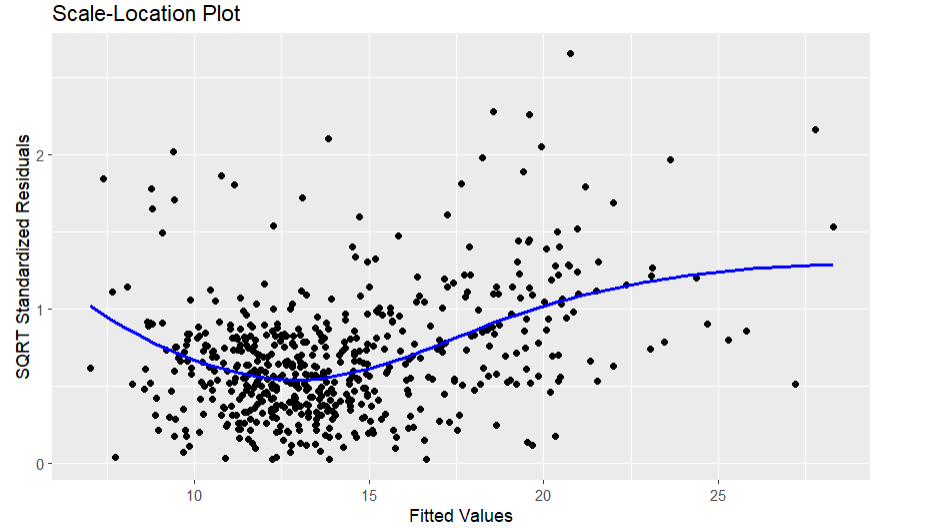
\epsfig{file = assets/mlr_scalelocation.png, width = 8 cm}}
      \caption{Scale-Location Plot}
      \label{fig:mlr_scale_location}
\end{figure}

\vspace{0.5cm}

The scale-location plot is a diagnostic plot used to assess  that the variance of the errors (or residuals) is constant across the range of fitted values.

We can observe from the plot \ref{fig:mlr_scale_location} that the smooth trend line, is not approximately horizontal.
The slight slope in the line may indicate that the variability of the residuals is not entirely constant but rather increases or decreases as the fitted values change. This could suggest a mild violation of the assumption that the variance of the residuals is constant across the range of fitted values.

\vspace{0.5cm}

\subsection{Logistic Regression}

In this subsection, we will present and discuss the results obtained for the final linear regression model.

The model summary output is as follows:

\begin{figure}[!h]
      \centering
       {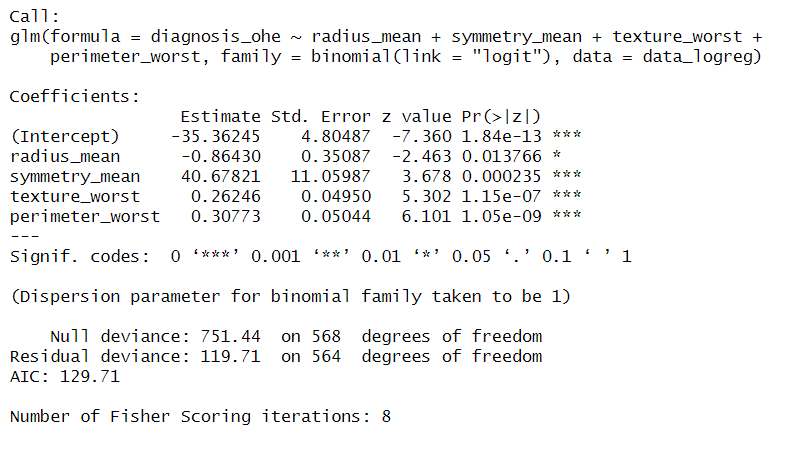
\epsfig{file = assets/logreg_final_summary.png, width = 8 cm}}
      \caption{Summary of the logistic regression model}
\end{figure}

\vspace{0.5cm}

The overall model suggests that the coefficients for all predictors have associated p-values that are less than the conventional significance level of 0.05. This indicates that all predictor variables are statistically significant in explaining the variability in the response variable (diagnosis). Therefore, we can infer that all predictors have statistically significant coefficients.

\vspace{0.5cm}

\textbf{Coefficients Interpretation}:
\begin{enumerate}
\item \textbf{Radius Mean:} For every one-unit increase in radius\_mean, the log odds of the diagnosis being malignant decrease by 0.86430 units, on average, holding other predictors constant.

\item \textbf{Symmetry Mean:} For every one-unit increase in symmetry\_mean, the log odds of the diagnosis being malignant increase by 40.67821 units, on average, holding other predictors constant.

\item \textbf{Texture Worst:}  For every one-unit increase in texture\_worst, the log odds of the diagnosis being malignant increase by 0.26246 units, on average, holding other predictors constant.

\item \textbf{Perimeter Worst:} For every one-unit increase in perimeter\_worst, the log odds of the diagnosis being malignant increase by 0.30773 units, on average, holding other predictors constant.

\end{enumerate}

\vspace{0.5cm}

The logistic regression model's adjusted hyperplane equation can be represented as follows:

\begin{equation}
\begin{aligned}
\text{logit}(\hat{p}) = &\quad -35.36245 \\
&\quad - 0.86430 \times \text{radius\_mean} \\
&\quad + 40.67821 \times \text{symmetry\_mean} \\
&\quad + 0.26246 \times \text{texture\_worst} \\
&\quad + 0.30773 \times \text{perimeter\_worst}
\end{aligned}
\end{equation}

\vspace{0.5cm}

The expression for p(x), which represents the probability of the outcome given the predictor variables x, can be derived from the logistic regression model using the sigmoid function:

\begin{equation}
\begin{aligned}
p(x)_{\text{logistic}} = \frac{1}{1 + e^{-\left(-35.36245 - 0.86430 \times \text{radius\_mean} +  \dotsb \right)}}
\end{aligned}
\end{equation}

\vspace{0.5cm}

\textbf{Odds ratios}
\begin{equation}
\begin{aligned}
OddsRatio_{x_i} = e^{\beta_i}
\end{aligned}
\end{equation}

\vspace{0.5cm}

\begin{figure}[!h]
      \centering
       {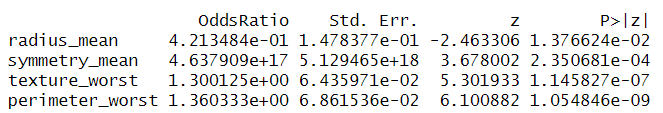
\epsfig{file = assets/oddsratios.png, width = 8 cm}}
      \caption{Odds ratios}
\end{figure}
\vspace{0.5cm}

The odds ratio indicates how the odds of the outcome change with a one-unit increase in the predictor variable, holding all other variables constant.
\vspace{0.5cm}

\textbf{Residuals Analysis}:

\begin{figure}[!h]
      \centering
       {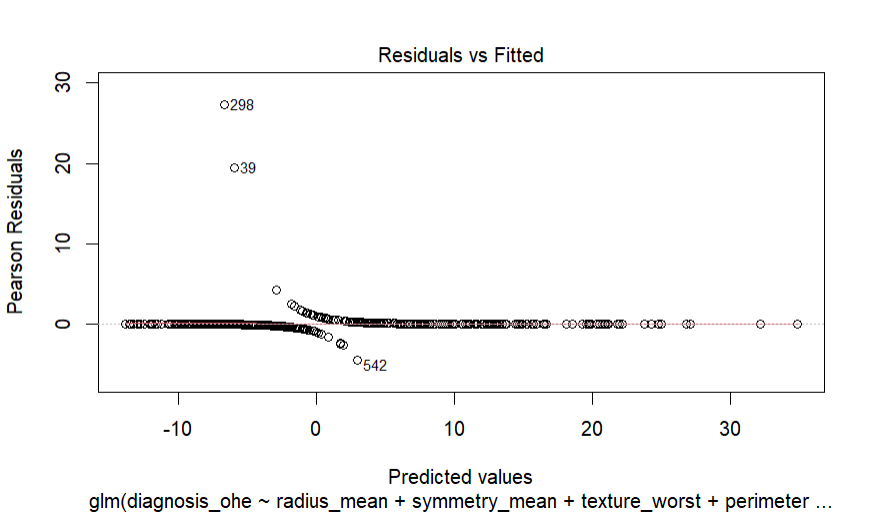
\epsfig{file = assets/log_residualsvsfitted.png, width = 8 cm}}
      \caption{Residuals vs. Fitted Values Plot}
      \label{fig:log_resvsfit}
\end{figure}

\vspace{0.5cm}

Upon examination of the residuals vs. fitted values plot, it is observed that the residuals exhibit a random dispersion around the horizontal line at y = 0, with some isolated exceptions. Furthermore, there is no discernible pattern evident in the residuals as the fitted values vary. Additionally, the spread of residuals remains relatively consistent across the spectrum of fitted values. These observations collectively suggest that the logistic regression model adequately captures the underlying relationship between the predictors and the response variable.

\vspace{0.5cm}
\begin{figure}[!h]
      \centering
       {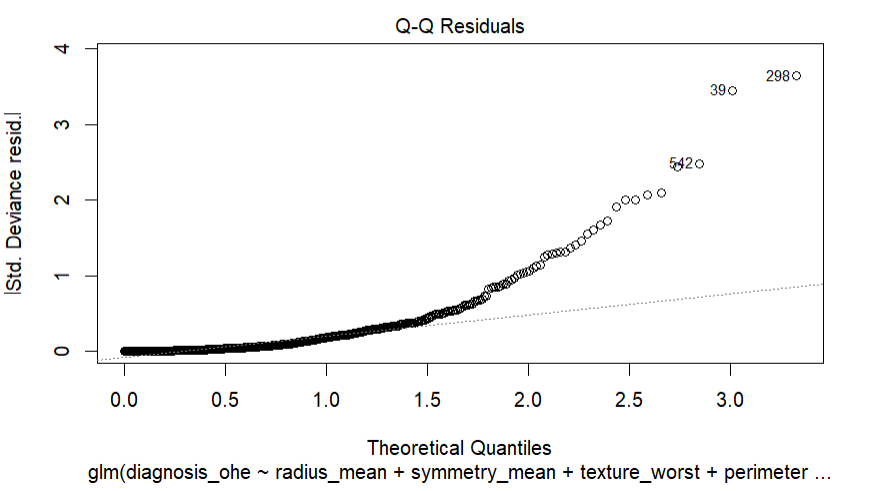
\epsfig{file = assets/log_qqplot.png, width = 8 cm}}
      \caption{Normal Q-Q Plot}
      \label{fig:log_qq}
\end{figure}
\vspace{0.5cm}

In the normal quantile-quantile (Q-Q) plot of the residuals, the observed residuals predominantly adhere to the theoretical quantiles, suggesting substantial conformity to the normal distribution assumption. However, a deviation from the expected pattern is noticeable at the right side of the quantiles axis. Despite this deviation, the overall assessment from the normal Q-Q plot suggests a reasonable level of adherence to normality for the residuals.

\vspace{0.5cm}
\begin{figure}[!h]
      \centering
       {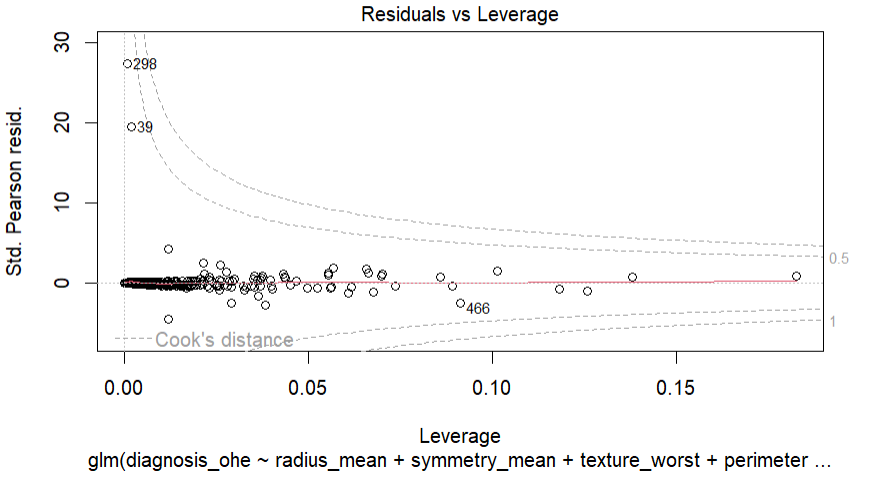
\epsfig{file = assets/log_std_res_vs_leverage.png, width = 8 cm}}
      \caption{Standardized Residuals vs. Leverage Plot}
      \label{fig:log_stdres_leverage}
\end{figure}
\vspace{0.5cm}

In a residuals vs. leverage plot, the leverage values represent the influence that each data point has on the estimation of the regression coefficients.

Overall, the plot exhibits a predominant clustering of points around the y = 0 line, with only minor instances of departure, indicative of a relatively well-behaved dataset with some slight outliers.

\vspace{0.5cm}

\begin{figure}[!h]
      \centering
       {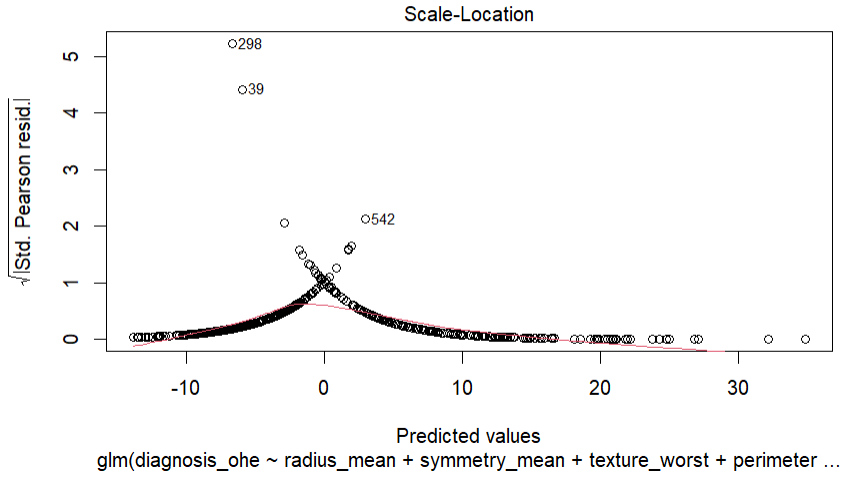
\epsfig{file = assets/log_scalevslocation.png, width = 8 cm}}
      \caption{Scale-Location Plot}
      \label{fig:log_scale_location}
\end{figure}
\vspace{0.5cm}

We can observe from the plot that the smooth trend line, is not approximately horizontal.
The slight slope in the line may indicate that the variability of the residuals is not entirely constant but rather increases or decreases as the fitted values change. This could suggest a mild violation of the assumption that the variance of the residuals is constant across the range of fitted values.
\subsection{Clustering}

Prior to presenting the results, it is pertinent to note that the features underwent scaling procedures before performing the clustering analysis.

\subsubsection{Hierarchical Clustering}
To analyze the optimal number of clusters for our data, we conducted a dendrogram analysis.
\vspace{0.5cm}
\begin{figure}[H]
      \centering
       {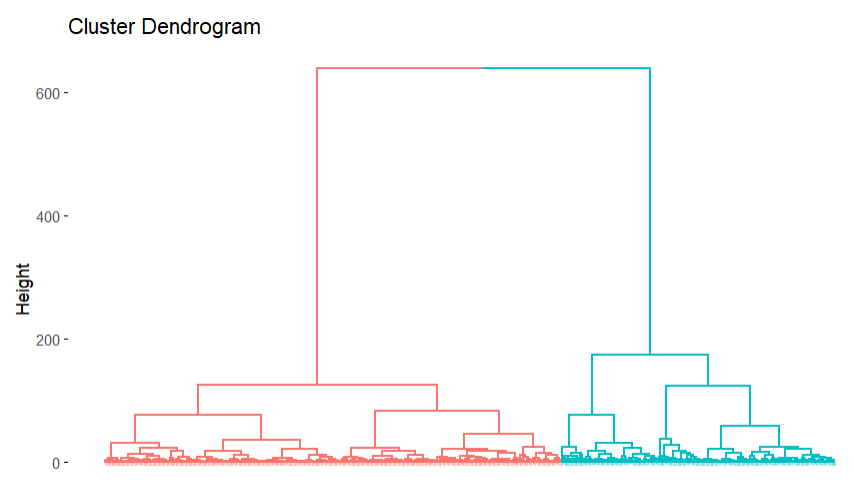
\epsfig{file = assets/dendrogram.png, width = 8 cm}}
      \caption{Dendrogram}
\end{figure}

Analyzing the dendrogram, we can ascertain that the most suitable number of clusters for our data is 2.

\vspace{0.5cm}

A visual representation of the hierarchical clusters:

\begin{figure}[H]
      \centering
       {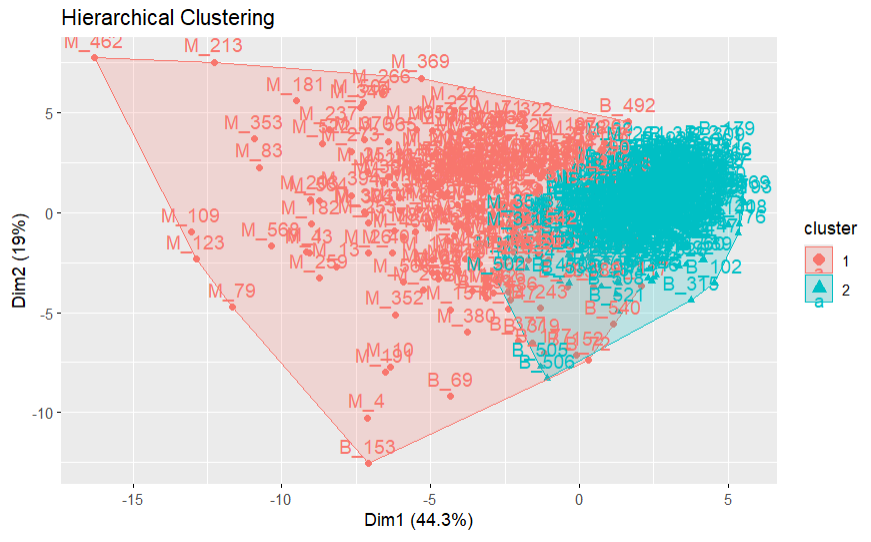
\epsfig{file = assets/h_clusters.png, width = 8 cm}}
      \caption{Hierarchical clusters}
\end{figure}


Mean and standard deviation for all variables by cluster.
The table is truncated, showing only a few features.

\begin{figure}[H]
      \centering
       {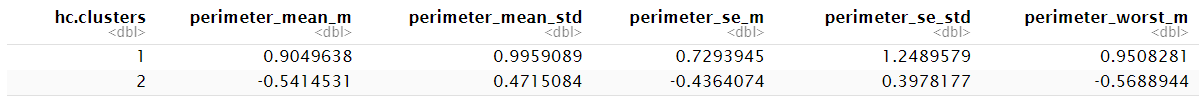
\epsfig{file = assets/m_std_h.png, width = 8 cm}}
      \caption{Mean and standard deviation by cluster}
\end{figure}

Comparison of cluster membership with diagnosis:
\begin{figure}[H]
      \centering
       {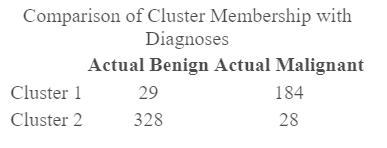
\epsfig{file = assets/h_membership.png, width = 8 cm}}
      \caption{Hierarchical Cluster vs. Actual Diagnosis}
\end{figure}


\subsubsection{K-means}

\vspace{0.5cm}

Regarding k-means clustering, we assessed the optimal
starting number of clusters (k) using the elbow method,
silhouette method, and clValid.

For illustrative purposes, we will present the graphical representation of the silhouette method.

\begin{figure}[H]
      \centering
       {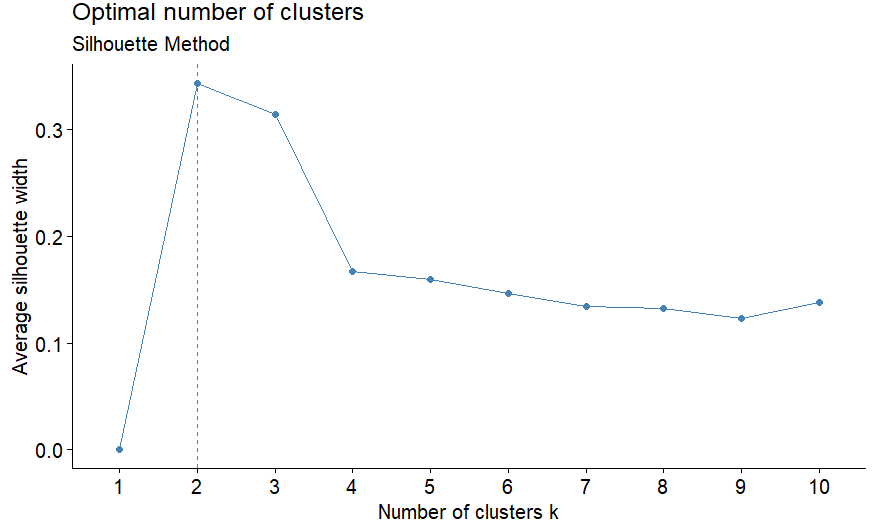
\epsfig{file = assets/silhouette.png, width = 8 cm}}
      \caption{Silhouette method}
\end{figure}


A visual representation of the k-means clusters:

\begin{figure}[H]
      \centering
       {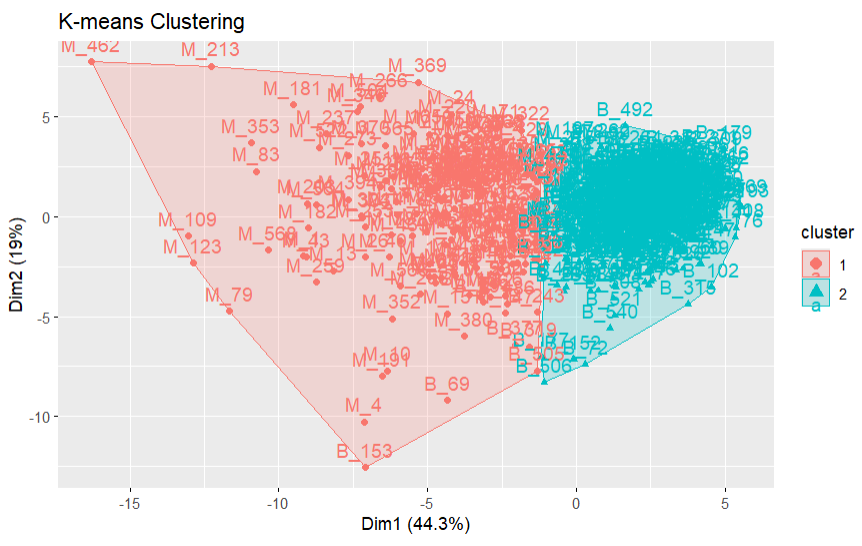
\epsfig{file = assets/kmeans_clusters.png, width = 8 cm}}
      \caption{K-means clusters}
\end{figure}

\begin{figure}[H]
      \centering
       {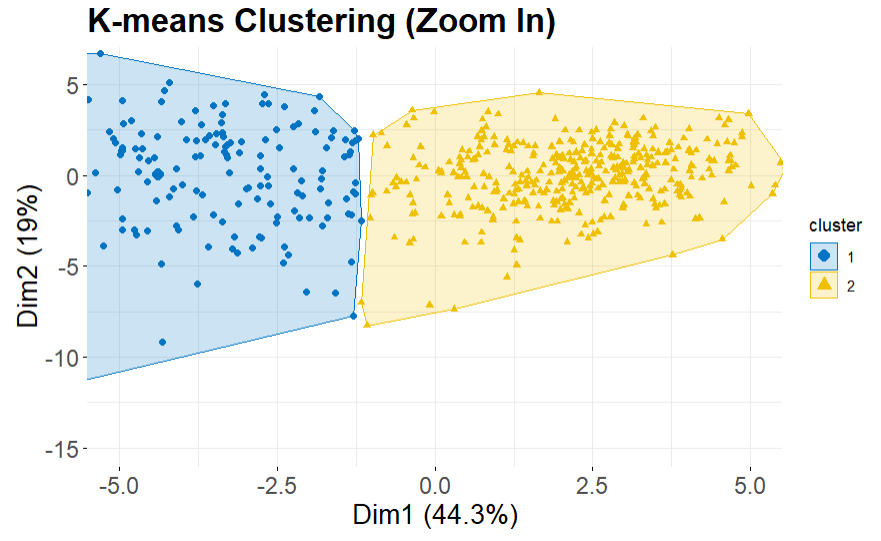
\epsfig{file = assets/kmeans_zoom.png, width = 8 cm}}
      \caption{K-means clusters (zoomed)}
\end{figure}

Mean and standard deviation for all variables by cluster.
The table is truncated, showing only a few features.

\begin{figure}[H]
      \centering
       {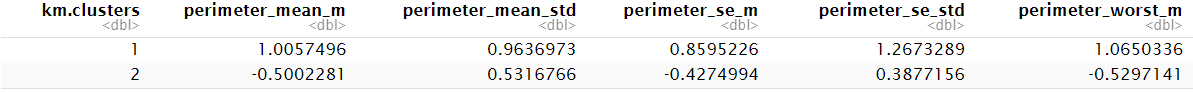
\epsfig{file = assets/kmeans_m_std.png, width = 8 cm}}
      \caption{Mean and standard deviation by cluster}
\end{figure}

Comparison of cluster membership with diagnosis:
\begin{figure}[H]
      \centering
       {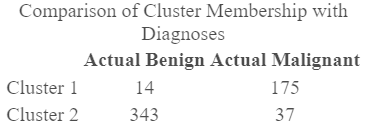
\epsfig{file = assets/k_means_membership.png, width = 8 cm}}
      \caption{K-means Cluster vs. Actual Diagnosis}
\end{figure}


\vspace{0.2cm}
\section{{Conclusion}}

In conclusion, the statistical analysis of the Wisconsin Breast Cancer dataset, incorporating linear regression, logistic regression, and clustering techniques, successfully achieved its objectives. Through these methodologies, significant insights were gleaned regarding the predictive factors and underlying structures associated with breast cancer, thereby enhancing our understanding of this complex disease and potentially informing future research and clinical practices.

\bibliographystyle{ieeetr}
\bibliography{citations}

\end{document}
